\documentclass[10pt, a4paper, twocolumn]{article}

% \usepackage[english]{babel} % English language hyphenation

% \usepackage{microtype} % Better typography

\usepackage{amsmath,amsfonts,amsthm} % Math packages for equations

\usepackage[svgnames]{xcolor} % Enabling colors by their 'svgnames'

\usepackage[hang, small, labelfont=bf, up, textfont=it]{caption} % Custom captions under/above tables and figures

\usepackage{booktabs} % Horizontal rules in tables

\usepackage{lastpage} % Used to determine the number of pages in the document (for "Page X of Total")

\usepackage{graphicx} % Required for adding images

\usepackage{enumitem} % Required for customising lists
\setlist{noitemsep} % Remove spacing between bullet/numbered list elements

% \usepackage{sectsty} % Enables custom section titles
%\allsectionsfont{\usefont{OT1}{phv}{b}{n}} % Change the font of all section commands (Helvetica)

%----------------------------------------------------------------------------------------
%	MARGINS AND SPACING
%----------------------------------------------------------------------------------------

\usepackage{geometry} % Required for adjusting page dimensions

\geometry{
	top=1cm, % Top margin
	bottom=1.5cm, % Bottom margin
	left=2cm, % Left margin
	right=2cm, % Right margin
	includehead, % Include space for a header
	includefoot, % Include space for a footer
	%showframe, % Uncomment to show how the type block is set on the page
}

\setlength{\columnsep}{7mm} % Column separation width

%----------------------------------------------------------------------------------------
%	FONTS
%----------------------------------------------------------------------------------------

% \usepackage[T1]{fontenc} % Output font encoding for international characters
% \usepackage[utf8]{inputenc} % Required for inputting international characters

%----------------------------------------------------------------------------------------
%	HEADERS AND FOOTERS
%----------------------------------------------------------------------------------------

\usepackage{fancyhdr} % Needed to define custom headers/footers
\pagestyle{fancy} % Enables the custom headers/footers

\renewcommand{\headrulewidth}{0.0pt} % No header rule
\renewcommand{\footrulewidth}{0.4pt} % Thin footer rule

\renewcommand{\sectionmark}[1]{\markboth{#1}{}} % Removes the section number from the header when \leftmark is used

%\nouppercase\leftmark % Add this to one of the lines below if you want a section title in the header/footer

% Headers
\lhead{} % Left header
\chead{\textit{\thetitle}} % Center header - currently printing the article title
\rhead{} % Right header

% Footers
\lfoot{} % Left footer
\cfoot{} % Center footer
\rfoot{\footnotesize Page \thepage\ of \pageref{LastPage}} % Right footer, "Page 1 of 2"

\fancypagestyle{firstpage}{ % Page style for the first page with the title
	\fancyhf{}
	\renewcommand{\footrulewidth}{0pt} % Suppress footer rule
}

%----------------------------------------------------------------------------------------
%	TITLE SECTION
%----------------------------------------------------------------------------------------

\newcommand{\authorstyle}[1]{{\large\usefont{OT1}{phv}{b}{n}\color{DarkRed}#1}} % Authors style (Helvetica)

\newcommand{\institution}[1]{{\footnotesize\usefont{OT1}{phv}{m}{sl}\color{Black}#1}} % Institutions style (Helvetica)

\usepackage{titling} % Allows custom title configuration

\newcommand{\HorRule}{\color{DarkRed}\rule{\linewidth}{1pt}} % Defines the gold horizontal rule around the title

\pretitle{
	\vspace{-30pt} % Move the entire title section up
	\HorRule\vspace{10pt} % Horizontal rule before the title
	\fontsize{32}{36}\usefont{OT1}{phv}{b}{n}\selectfont % Helvetica
	\color{DarkRed} % Text colour for the title and author(s)
}

\posttitle{\par\vskip 15pt} % Whitespace under the title

\preauthor{} % Anything that will appear before \author is printed

\postauthor{ % Anything that will appear after \author is printed
	\vspace{10pt} % Space before the rule
	\par\HorRule % Horizontal rule after the title
	\vspace{20pt} % Space after the title section
}

%----------------------------------------------------------------------------------------
%	ABSTRACT
%----------------------------------------------------------------------------------------

\usepackage{lettrine} % Package to accentuate the first letter of the text (lettrine)
\usepackage{fix-cm}	% Fixes the height of the lettrine

\newcommand{\initial}[1]{ % Defines the command and style for the lettrine
	\lettrine[lines=3,findent=4pt,nindent=0pt]{% Lettrine takes up 3 lines, the text to the right of it is indented 4pt and further indenting of lines 2+ is stopped
		\color{DarkRed}% Lettrine colour
		{#1}% The letter
	}{}%
}

\usepackage{xstring} % Required for string manipulation

\newcommand{\lettrineabstract}[1]{
	\StrLeft{#1}{1}[\firstletter] % Capture the first letter of the abstract for the lettrine
	\initial{\firstletter}\textbf{\StrGobbleLeft{#1}{1}} % Print the abstract with the first letter as a lettrine and the rest in bold
}



\hbadness=10000
% TITLE PAGE
\title{PHYS 260 Electromagnetism}
\author{\authorstyle{Miles Kent}}
\date{}
\begin{document}
\graphicspath{ {./images/} }

\maketitle

\textbf{\huge Chapters 21-22}
    \section{Electrostatics Basics}    
        \subsection{Introduction}
            \begin{enumerate}
                \item {
                    As you may know, matter is made of atoms.
                    Atoms have a nucleus, which is made up of protons (positive) and neutrons (neutral), and electrons (negative).
                    Opposite charges are attracted to one another with a inverse square force, and like charges are similarly repelled.
                }
                \item {
                    The electrons\footnote{Not \textit{all} of the electrons in a conductor can move, it's just that the ones that don't move can be ignored because they do not contribute to the net charge of a material} in conductors are able to move freely, while in insulators they cannot unless they come off entirely
                }
                \item {
                    Some materials tend to give off electrons (e.g. fur) and some tend to attract them (e.g. plastic)   
                }
                \item {
                    Not all metals are conductors
                }
                \item {
                    A neutral object can be attracted to a charged object via inducted polarity. In a conductor, this means the electrons move through the entire object to create a dipole. In an insulator, the electrons of the atoms realign to create billions of of tiny dipoles. This makes a difference due to the inverse square law, which will be discussed further later. The former creates a strong attraction, while the latter creates a weak attraction.
                }
            \end{enumerate}
        \subsection{Electrical Grounding}
            An object can be "grounded" by connecting it to a big conductor, which serves as a resevoir for charge, e.g. you can ground the wall outlet by sticking a fork into it. The gruond in this case is you body and the ground. The electricity from the wall will flow through your body and into the ground


    \section{Coulomb's Law}    
        The magnitude of the force between two point charges $q_1$ and $q_2$ C, with distance $r$ m is equal to the following
        \begin{align*} 
            F = \frac{1}{4\pi \epsilon_0} \frac{|q_1 \cdot q_2|}{r^2}
        \end{align*} 
        \begin{itemize}
            \item where $\epsilon_0$ is vacuum permittivity, the value of the absolute dielectric permittivity of classical vacuum, or also just "the electric constant".  
            \item $\epsilon_0 \approx 8.854189 \cdot 10^{-12}$ 
            \item the Coulomb constant $k = \frac{1}{4\pi \epsilon_0}$
            \item electric forces add as vectors, which is called the "Superposition Principle"
        \end{itemize}


    \section{Electric Fields}
        \begin{itemize}
            \item Electric Fields are best represented by vector fields

            \item For the electric field of a point charge\\ $\vec{F} = q \vec{E} \rightarrow E = \frac{F}{q} \rightarrow E = \frac{1}{4\pi \epsilon_0} \frac{q}{r^2} = \frac{kq}{r^2}\ \frac{N}{C}$

            \item Field lines do not indicate the trajectory of a test charge, but rather are lines tangent to the electric field at a given point
        \end{itemize}

        \subsection{Electric Field Integrations}    
            As it turns out, it is unrealistic to use Coulomb's Law just by itself to calculate the electric field at a point. This would require knowing the location and charge of every charge in an object. One way this problem can be simplified is with the use of charge density and calculus. 
            \begin{itemize}
                \item Linear density: $\lambda = \frac{Q}{L}$
                \item Area density: $\sigma = \frac{Q}{A}$
                \item Volumetric density: $\rho = \frac{Q}{V}$
            \end{itemize}

            Basically, what you do is find the ds/dA/dV and you multiply it times the charge density to get the dQ. You then usually use the point charge electric field formula and integrate it over the relevant domain. When the differential is a point charge, you usually need to make sure you aren't summing magnitudes. However, if the differential you are given is an area, this has probably already been taken care of.\\

            \textbf{Infinite Sheet of Charge}
            $$|\vec{E}| = \frac{\sigma}{2\epsilon_0}$$\\

        \textbf{\footnote{The field due to \textit{everything}}{Near the Surface of a Conductor}}
            $$|\vec{E}| = \frac{\sigma}{\epsilon_0}$$\\

    \section{Gauss' Law}
    $$\Phi = \oint \vec{E} \cdot d\vec{A} = \oint \vec{E} \cdot \hat{n}\ dA = \frac{Q_{net}}{\epsilon_0}$$\\
    The above equation is Gauss' Law, which states that the flux through a surface is a measure of how orthogonally an electric field passes through a surface. Positive flux means that the passing it outward, while negative flux means that it is inward (overall). Finding flux is useful because it is proportional to the net charge of within the surface of the integral. The surface used in the integral typically is not a real surface, but a contrived one, used for determining the net charge of what it encloses. It is called a Gaussian Surface and is usually a rectangular prism, cylinder, or sphere, depending on what is most convienient.\\ \\
    Furthermore, if the electric field is uniform and the angle between the field and the surface is constant, then the following applies.\\
    $$\Phi = \vec{E} \cdot \vec{A} = EAcos(\theta) = \frac{Q_{net}}{\epsilon_0}$$\\ 
    where $\theta$ is the angle between the electric field and the normal vector $\hat{n}$\\

        \subsection{Flux}
        Based on the previous simplified equation, it becomes obvious that the units of flux are $\frac{N}{C} \cdot{m^2}$. If you think about the electric field as the flowing of water, in a river perhaps, then flux is like a measure of that flow times an area, i.e. a rate of volume. Obviously, an electric field is, in fact, not flowing water, but this analogy is useful.


    \section{Dipoles}    
    $\vec{p} = q \vec{d}$\\
    $\vec{\tau} = \vec{p} \times \vec{E}$\\
    $|\vec{\tau}| = pEsin(\theta)$\\
    $W = \int^{\phi_2}_{\phi_1} (-pEsin(\phi))d\phi = pE(cos(\phi_2) - cos(\phi_1))$
    $U(\phi) = -\vec{p} \cdot \vec{E} = -pEcos(\phi)$\\ \\

\textbf{\huge Chapters 23-25}
% 23
    \section{Electric Potential Energy}	
        Recall: Work done by a conservative force is equal to the following
        $$W_{a\rightarrow b} = -\Delta U$$
        Recall: Electrostatic force
        $$F_e = qE$$
        Therefore, in a uniform electric field between parallel plates
        $$U = (qE)y$$
        $$W_{a \rightarrow b} = F_e d = (qE)\delta y$$
        For a point charge
        $$F = \frac{1}{4 \pi \epsilon_0} \frac{q q_0}{r^2}$$
        $$U = \frac{1}{4 \pi \epsilon_0} \frac{q q_0}{r}$$
        Superposition applies
        $$U = \frac{q_0}{4 \pi \epsilon_0} \Sigma_{i} \frac{q_i}{r_i}$$

    \section{Electric Potential}	
        Potential is just potential energy per unit charge
        $$V = \frac{U}{q_0}$$
        $$U = q_0 V$$
        The units are volts ($V$, $\frac{J}{C}$)
        The potential difference $\Delta V$ is also called voltage. It is equal to the work in joules that must be done to move a 1 couloumb charge from a to b against the electric force.
        $$\frac{W_{a \rightarrow b}}{q_0} = \frac{-\Delta U}{q_0} = -\Delta V$$
        Usually since a and b are arbitrary, the voltage is usually given as an absolute value\\
        A 9V battery has a potential difference or voltage of 9V which means that the difference between the positive and negative terminals is 9V\\
        The electric potential due to a point charge:
        $$V = \frac{1}{4 \pi \epsilon_0} \frac{q}{r} = \frac{U}{q_0}$$
        Accordingly:
        $$V = \frac{1}{4 \pi \epsilon_0} \Sigma_{i} \frac{q_i}{r_i}$$
        $$V = \frac{1}{4 \pi \epsilon_0} \int \frac{dq}{r}$$
        The electric potential due to a field $\vec{E}$
        $$W_{a \rightarrow b} = \int^{b}_{a} \vec{F} \cdot d \vec{l} = \int^{b}_{a} q_0 \vec{E} \cdot d \vec{l}  $$
        Divide by $q_0$
        $$-\Delta V = \int^{b}_{a} \vec{E} \cdot d \vec{l} = \int^{b}_{a} Ecos\phi\ dl  $$
        ito $\vec{E}$ we get:
        $$\vec{E} = -\nabla V$$
        Think of just
        $$-\Delta V = \int^{b}_{a} E_x dx$$
        $$-\int^{b}_{a} dV = \int^{b}_{a} E_x dx$$
        $$-dV = E_x dx$$
        $$-\frac{dV}{dx} = E_x$$
        If you do for y, z then you get negative gradient

    \section{Equipotential Surfaces}	
        Equipotential surfaces for electric fields can be entirely generalized to the idea of a topographical map.
        \begin{figure}[H]
            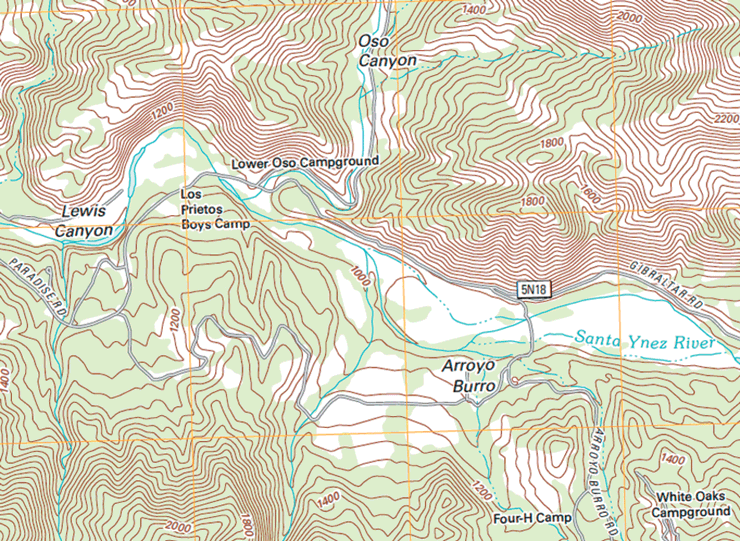
\includegraphics[width=\linewidth]{topo-map} % Figure image
            \caption{Topographical map} % Figure caption
        \end{figure}

        Because of $\vec{E} = -\nabla V$, given that the topographical lines are like potential lines, the field lines are perpindicular and in the downhill direction. These could be imagined as the lines of errosion. 

% 24
    \section{Capacitors and Capacitance}	
    Any two conductors separated by an insulator (or \footnote{vaccuum}{i.e. not a conductor})
    \section{Capitors in Series and Parallel}	
    \section{Energy in a Capacitor}	
    \section{Dielectrics}	
% 25
    \section{Current \& Current Density}	
    \section{Resistivity}	
    \section{Resistors}	
    \section{Circuits and EMF}	
        EMF $\Delta V$ is $\mathcal{E}$
    \section{Energy \& Power in Circuits}	
    \section{Conduction in Metals}	
% 26
    \section{Resistors in Series and Parallel}
    \section{Kirchhoff's Rules}
    \section{Electrical Measuring Instruments}
    \section{R-C Circuits}
    \section{Power Distribution Systems}

\end{document}
